\documentclass[12pt]{report}

\usepackage[a4paper, total={17cm, 24cm}]{geometry}
\usepackage{exercise}
\usepackage{tikz}
%\usetikzlibrary{positioning,external}
%\tikzexternalize[prefix=tikz/]
%\usetikzlibrary{scopes}
%\usetikzlibrary{backgrounds}


\renewcommand{\ExerciseHeader}{\noindent\textbf{\large\ExerciseName\ %
\ExerciseHeaderNB\ExerciseHeaderTitle
\ExerciseHeaderOrigin\medskip}}
\setlength{\QuestionIndent}{1.5em}

\newcommand{\answerbox}[2]{\hfill\break\\
        \framebox[\linewidth]{\parbox[c][#1][c]{\dimexpr\linewidth-2\fboxsep-2\fboxrule}{#2}}
}

\renewcommand{\arraystretch}{1.2} % vertical padding for tabular environment

\begin{document}

\hfill
\begingroup
\Large
\begin{tabular}{|l|p{6cm}|}
	\hline
	First \& last name &
	% YOUR NAME HERE
	\\ \hline
	NOMA UCLouvain & 
	% YOUR NOMA HERE
	\\ \hline
\end{tabular}
\endgroup
\vspace{1.5cm}

\noindent
\begingroup
	\Large
	\textbf{LINFO2266: Advanced Algorithms for Optimization}\\\\
	Project 2: Branch and Bound
\endgroup
\vspace{0.2cm}

\begin{Exercise}[title={Modeling the Traveling Salesman Problem}]

\begin{center}
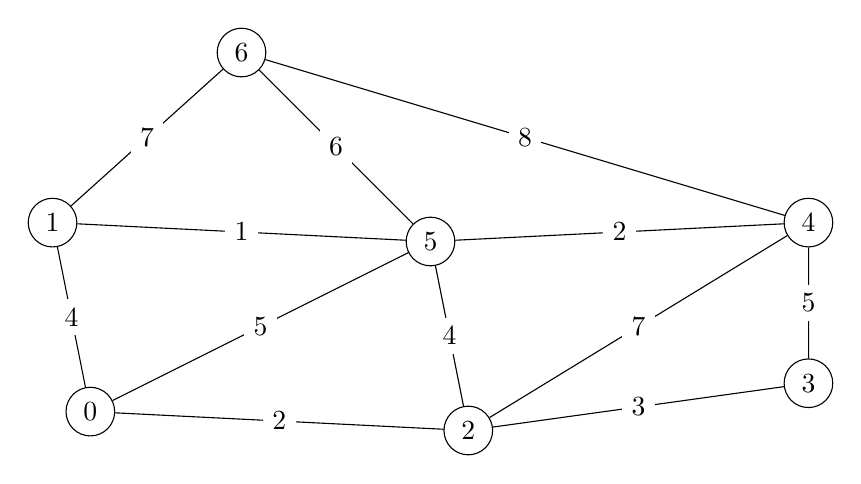
\begin{tikzpicture}[scale=1.2]
	\node[draw,circle] (v0) at (0.4,0.2) {0};
	\node[draw,circle] (v1) at (0,2.2) {1};
	\node[draw,circle] (v2) at (4.4,0) {2};
	\node[draw,circle] (v3) at (8,0.5) {3};
	\node[draw,circle] (v4) at (8,2.2) {4};
	\node[draw,circle] (v5) at (4,2) {5};
	\node[draw,circle] (v6) at (2,4) {6};
	
	\draw (v0) edge node[fill=white] {4} (v1);
	\draw (v0) edge node[fill=white] {2} (v2);
	\draw (v0) edge node[fill=white] {5} (v5);
	\draw (v1) edge node[fill=white] {1} (v5);
	\draw (v1) edge node[fill=white] {7} (v6);
	\draw (v2) edge node[fill=white] {3} (v3);
	\draw (v2) edge node[fill=white] {7} (v4);
	\draw (v2) edge node[fill=white] {4} (v5);
	\draw (v3) edge node[fill=white] {5} (v4);
	\draw (v4) edge node[fill=white] {2} (v5);
	\draw (v4) edge node[fill=white] {8} (v6);
	\draw (v5) edge node[fill=white] {6} (v6);
\end{tikzpicture}
\end{center}

\Question Explain and depict with the help of the visual example your internal state representation and your successor function for the TSP.
\answerbox{10cm}{
% YOUR ANSWER HERE
}


\end{Exercise}

\begin{Exercise}[title={One-tree lower-bound}]

\Question What is your strategy to avoid including the excluded edges in your implementation
of the one-tree relaxation.
\answerbox{10cm}{
% YOUR ANSWER HERE
}


\Question Give the timple-complexity and justify your answer (don't forget to specify the spanning tree algorithm that you use)
\answerbox{6cm}{
% YOUR ANSWER HERE
}


\end{Exercise}

\pagebreak


\begin{Exercise}[title={Held and Karp lower-bound}]

\Question For the instance \verb|instance_30_0.xml| make a plot of the evolution of the lower-bound along the iterations of the gradient descent. The x-axis should have the iterations, and the y-axis the value of the lower-bound.
\answerbox{12cm}{
% YOUR ANSWER HERE
}


\Question What do you observe, conclude ? How can this plot help you to tune the parameters of the Held-Karp lower-bound algorithm.
\answerbox{6cm}{
% YOUR ANSWER HERE
}


\end{Exercise}

\end{document}